\documentclass[11pt]{article}
\usepackage[T1]{fontenc}
\usepackage{lmodern}
\usepackage[margin=1in]{geometry}
\usepackage{amsmath,amssymb,amsthm,mathtools}
\usepackage{microtype,booktabs,array,longtable,graphicx}
\usepackage{xcolor}
\usepackage[unicode,colorlinks=true,linkcolor=blue!45!black,urlcolor=blue!55!black,citecolor=blue!45!black]{hyperref}
\usepackage{enumitem}
\usepackage{fancyhdr}
\usepackage{listings}
\definecolor{navy}{RGB}{24,48,75}
\definecolor{teal}{RGB}{0,104,112}
\definecolor{lightgray}{RGB}{246,248,250}
\hypersetup{pdftitle={A factorial Cauchy expansion for the subexponential 3-SAT algorithm},pdfauthor={Research analysis prepared for Vladimir Reshetnikov}}
\pagestyle{fancy}
\fancyhf{}
\fancyhead[L]{\small\sffamily Factorial Cauchy modes for 3-SAT}
\fancyhead[R]{\small\sffamily Research note}
\fancyfoot[C]{\small\thepage}
\setlength{\headheight}{14pt}
\setlength{\parskip}{0.35em}
\setlength{\parindent}{0pt}
\setlength{\emergencystretch}{2em}
\allowdisplaybreaks[2]
\newtheorem{theorem}{Theorem}[section]
\newtheorem{lemma}[theorem]{Lemma}
\newtheorem{proposition}[theorem]{Proposition}
\newtheorem{corollary}[theorem]{Corollary}
\theoremstyle{remark}
\newtheorem{remark}[theorem]{Remark}
\newcommand{\OO}{\mathcal O}
\newcommand{\vv}{v_2}
\newcommand{\sbit}{s_2}
\newcommand{\poly}{\operatorname{poly}}
\newcommand{\polylog}{\operatorname{polylog}}
\newcommand{\Ztwo}{\mathbb Z_{(2)}}
\newcommand{\CP}{\mathcal C}
\newcommand{\qedstatus}[1]{\textbf{Status.} #1}
\lstset{basicstyle=\small\ttfamily,breaklines=true,columns=fullflexible,backgroundcolor=\color{lightgray},frame=single,rulecolor=\color{black!15},xleftmargin=0.5em,xrightmargin=0.5em}
\title{\vspace{-1em}\color{navy}\LARGE A factorial Cauchy expansion for the\newline subexponential 3-SAT algorithm\par\vspace{0.5em}\large A provable improvement of the enumeration exponent,\newline with precise limits on the resulting complexity claim}
\author{Research analysis prepared for Vladimir Reshetnikov}
\date{October 26, 2026}
\begin{document}
\maketitle
\thispagestyle{empty}
\begin{abstract}
We propose a replacement for the geometric-series modes in the tensor-contraction appendix of OpenAI's October 25, 2026 manuscript \emph{The Exponential Time Hypothesis is False}. An exact finite Cauchy separation, with integral source functions and factorial factors transferred into the target coefficients, changes the certified mode weights from $b+1$ to
\[
 w_b=1+b+2v_2(b!)=3b+1-2s_2(b).
\]
The same column tiles and source/target groups are used. Consequently the leading logarithm of the abstract mode-tuple count decreases by a factor $1/\sqrt3$. We prove the identity, the necessary integrality statement at the manuscript's unramified-extension interpolation points, compatibility with its recursion, and a sharper explicit running-time upper bound for matched contraction parameters. Exact rational and modular prototype checks accompany the analysis.

This is a constant-factor improvement \emph{inside a growing exponential}, rather than a new power of $\log n$: the general-CNF order remains $\poly(n,m)2^{O(n\log\log n/\sqrt{\log n})}$. No stronger order bound, complete optimized SAT implementation, or Lean formalization of the new lemmas is claimed. The results depend on the correctness of the manuscript's unchanged contraction and reduction arguments.
\end{abstract}
\vfill
\begin{center}\small
Source snapshot: \texttt{openai/math}, commit\par
\texttt{7ef5c0cc5ca4b0e072b7a050fca09ab24bc6fa3a}.\par
The accompanying archive contains this source, its compiled PDF,\par
an executable kernel prototype, verification results, and exact mode counts.
\end{center}
\clearpage
\tableofcontents
\clearpage

\section{What is improved, and what remains open}

The strongest justified proposal in this analysis is a change of basis in the paper's expensive mode enumeration. The change improves a specified exponential upper-bound coefficient while preserving exact counting, deterministic execution, and polynomial working space. It does not establish a bound such as $2^{O(n/(\log n)^{2/3})}$, or remove the $\log\log n$ factor for arbitrary clause density. Those would require further results.

\subsection{The source and the comparison baseline}

The source manuscript gives, for fixed clause width, the bounds
\begin{align}
 T_{\mathrm{general}}(n,m)&=(n+m)^{O(1)}
       2^{O(n\log\log n/\sqrt{\log n})},\label{eq:baseline-dense}\\
 T_{\mathrm{sparse}}(n,m)&=(n+m)^{O(1)}
       2^{O(n/\sqrt{\log n})}\quad(m=O(n)).\label{eq:baseline-sparse}
\end{align}
Its scope document separately states that the released Lean formalization covers the weaker general exponent $O(n(\log\log n)^2/\sqrt{\log n})$ \cite{paper,scope}. These are three distinct statements; our comparison uses the sharper manuscript construction, not the weaker formalized bound.

The target folder contains a PDF, a README, and four LaTeX files. This work studies the algorithm specified there. The accompanying code implements the replacement kernel and its tests, not an end-to-end executable reconstruction of every component of the paper. Source identifiers and verified Git blob hashes are recorded in \texttt{source\_manifest.json}.

\subsection{A precise meaning of the speedup}

Let $c$ be the number of column-tile families and $p$ a precision budget. If $\mathcal N_1(p,c)$ counts the nonnegative mode-exponent tuples with geometric weights $b+1$, and $\mathcal N_3(p,c)$ counts them with the new weights, then, in the growing-precision regime specified in Section~\ref{sec:entropy},
\begin{equation}\label{eq:headline-entropy}
 \log\mathcal N_3(p,c)
 =\left(\frac1{\sqrt3}+o(1)\right)\log\mathcal N_1(p,c).
\end{equation}
Equivalently, the new abstract enumeration has size $\mathcal N_1^{1/\sqrt3+o(1)}$. Its savings are exponential in $\sqrt{cp}$, rather than merely a constant multiplicative reduction in running time.

There are two qualifications. First, tuple counts are not measured SAT runtimes: many tuples may yield zero, and other work must be included. Second, the source states its main bounds with unspecified $O$-constants. We cannot divide an unknown source constant by $\sqrt3$ and call that a new published theorem. Section~\ref{sec:global} instead derives two \emph{explicit, matched} upper bounds, one for each mode basis. Their leading coefficients have exactly this ratio.

\begin{center}
\begin{tabular}{@{}lll@{}}
\toprule
Mode basis & Certified weight at index $b$ & Leading entropy ratio\\
\midrule
Geometric & $b+1$ & $1$\\
One-sided Newton & $b+1+v_2(b!)$ & $1/\sqrt2$\\
Factorial Cauchy & $b+1+2v_2(b!)$ & $1/\sqrt3$\\
\bottomrule
\end{tabular}
\end{center}
The Newton basis is a useful intermediate check. The factorial Cauchy basis is the recommended replacement.

\section{The interface to the existing contraction algorithm}\label{sec:interface}

We isolate the assumptions needed from the source, so the proposed change can be reviewed independently. The notation below describes one recursive contraction call; it is not a new proof of the entire source theorem.

Let $M$ be the number of Boolean wires. The paper packs their ports into packets with $L=2^a$ slots, and introduces the polynomial kernel
\begin{equation}\label{eq:paper-kernel}
 W_{xy}(T)=\frac{\CP(T)}{\CP'(0)(T-(y-x))},\qquad
 \CP(T)=\prod_{q=-L}^{L-1}(T-q).
\end{equation}
At a retained nonzero node $t$, write $i=v_2(t)$. Evaluation occurs at
\[
 T=t+2^{a+1}\zeta,\qquad \zeta\in\OO,
\]
where $\OO$ is the source's unramified extension of $\Ztwo$. Its valuation is normalized by $v_2(2)=1$. The residue field can be larger than $\mathbb F_2$, which will matter below.

Columns in a tile have slot positions
\[
 y=y_0+2^{i+1}j,\qquad 0\le j<J,
 \qquad D=2^{a-i},\qquad J=D/2.
\]
Only real ports contribute to a source linear form; the full interval describes all possible slot indices. For every crossing row $x$, the source construction supplies
\begin{equation}\label{eq:source-crossing-facts}
 d_0=t-y_0+x\ne0,\quad v_2(d_0)\le i,\quad
 v_2\!\left(\frac{\CP(T)}{\CP'(0)}\right)\ge a+1.
\end{equation}
Define
\begin{equation}\label{eq:normalized-kernel}
 d_x=d_0+2^{a+1}\zeta,\quad
 z_x=\frac{2^{i+1}}{d_x},\quad
 c_x=\frac{\CP(T)}{\CP'(0)d_x}.
\end{equation}
Then $z_x\in2\OO$, $c_x\in2\OO$, and the crossing entry is simply
\begin{equation}\label{eq:normalized}
 W_{xy}(T)=\frac{c_x}{1-z_xj}.
\end{equation}
The original mode expansion uses powers $j^b$ and row coefficients $c_xz_x^b$, assigning the uniform weight $b+1$. There are at most $6M/D$ tile families. The precision at this node is bounded on the scale $MD/u$, where $u$ is the retained valuation-level parameter. These facts are the interface from the source's contraction appendix \cite{contraction}.

The task is to separate \eqref{eq:normalized} into integral functions of $x$ and $j$, with better divisibility in the $x$ factor, without creating additional tile families. A mere rewriting that divides by factorials in the source factors would not suffice: it could cancel the divisibility we want to exploit.

\section{An exact finite Cauchy separation}\label{sec:identity}

For $b\ge0$, put
\begin{align}
 A_b(z)&=\prod_{h=0}^{b-1}\frac{z-2h}{1-hz},&
 B_b(j)&=\prod_{h=0}^{b-1}\frac{j-h}{1-2hj},\label{eq:AB}\\
 Q_b(z,j)&=\frac{(1-2b^2)A_b(z)B_b(j)}{(1-bz)(1-2bj)}.
 \label{eq:Q}
\end{align}
An empty product is one. All the displayed denominators are units when $z\in2\OO$ and $j$ is an ordinary integer.

\begin{lemma}[Finite separation with explicit remainder]\label{lem:identity}
For every nonnegative integer $q$,
\begin{equation}\label{eq:finite-separation}
 \frac1{1-zj}
 =\sum_{b=0}^{q-1}Q_b(z,j)
    +\frac{A_q(z)B_q(j)}{1-zj}.
\end{equation}
In particular, if $0\le j<J$, then
\begin{equation}\label{eq:exact-J}
 \frac1{1-zj}=\sum_{b=0}^{J-1}Q_b(z,j).
\end{equation}
\end{lemma}

\begin{proof}
Let $R_b=A_b(z)B_b(j)/(1-zj)$. From \eqref{eq:AB},
\[
 \frac{R_{b+1}}{R_b}
 =\frac{(z-2b)(j-b)}{(1-bz)(1-2bj)}
\]
whenever the quotient is meaningful, and the corresponding cross-multiplied identity always holds. The elementary identity
\[
 (1-bz)(1-2bj)-(z-2b)(j-b)
 =(1-2b^2)(1-zj)
\]
therefore gives $R_b-R_{b+1}=Q_b$. Telescope from $b=0$ to $q-1$, using $R_0=1/(1-zj)$. If $q=J$ and $j<J$, the product defining $B_J(j)$ contains the factor $j-j$, so the remainder is exactly zero.
\end{proof}

This identity is finite and algebraic. There is no analytic convergence assumption and no infinite-series error to estimate. It can also be viewed as Cauchy elimination at auxiliary row points $z=2b$ and column points $j=b$. The auxiliary row points need not be real rows of a packet.

\subsection{Moving both factorial gains into the target}

Define the source function
\begin{equation}\label{eq:source-feature}
 \ell_b(j)=
 \frac{(1-2b^2)\binom jb}{\prod_{h=0}^{b}(1-2hj)},
 \qquad \binom jb=0\ \text{when }b>j,
\end{equation}
and the target coefficient
\begin{equation}\label{eq:target-feature}
 r_b(x)=c_x\,b!\,
 \frac{A_b(z_x)}{1-bz_x}.
\end{equation}
Because $\prod_{h<b}(j-h)=b!\binom jb$, Lemma~\ref{lem:identity} yields
\begin{equation}\label{eq:main-separation}
 \boxed{\displaystyle
 W_{xy}(T)=\sum_{b=0}^{J-1}r_b(x)\ell_b(j).}
\end{equation}
The source function lies in $\Ztwo$: its denominator is an odd integer. The second factorial is multiplied into $r_b$, rather than implemented by a nonunit division. The remaining question is the valuation of $A_b(z_x)$ in the extension ring.

\section{The integrality lemma that makes the improvement valid}\label{sec:integrality}

It would be incorrect to assert that $\binom wb$ belongs to $\OO$ for every $w\in\OO$. For example, a residue $U\in\mathbb F_4\setminus\mathbb F_2$ need not make $U(U-1)$ divisible by two. The actual interpolation rows obey a much stronger congruence.

\begin{lemma}[Factorial divisibility near the prime subring]\label{lem:factorial}
Suppose $w,w_0\in\OO$, $w_0\in\Ztwo$, and
\[
 w-w_0\in2^R\OO.
\]
If $0\le b<2^R$, then
\begin{equation}\label{eq:factorial-divisibility}
 v_2\!\left(\prod_{h=0}^{b-1}(w-h)\right)\ge v_2(b!).
\end{equation}
\end{lemma}

\begin{proof}
For every $1\le r\le\lfloor\log_2 b\rfloor$, the rational $2$-integral number $w_0$ has an ordinary integer residue modulo $2^r$. Among $b$ consecutive integers, at least $\lfloor b/2^r\rfloor$ have that residue. For those $h$, both $w_0-h$ and $w-w_0$ are divisible by $2^r$, because $r\le R$. Thus the same divisibility holds for $w-h$. Sum the contributions over $r$, counting a factor again for each additional power of two it contains. The result is
\[
 \sum_{r\ge1}\left\lfloor\frac b{2^r}\right\rfloor=v_2(b!).
\]
The cases $b=0,1$ are immediate. A zero factor only increases the valuation.
\end{proof}

\begin{lemma}[The source interpolation values satisfy the congruence]\label{lem:actual-domain}
For a crossing row from Section~\ref{sec:interface}, put $w=z_x/2$ and $w_0=2^i/d_0$. Then $w_0\in\Ztwo$ and
\begin{equation}\label{eq:prime-congruence}
 w-w_0\in2^{a+1-i}\OO.
\end{equation}
Consequently $v_2(A_b(z_x))\ge b+v_2(b!)$ for every $0\le b<J$.
\end{lemma}

\begin{proof}
Let $d=v_2(d_0)\le i$. Adding $2^{a+1}\zeta$ does not change this valuation. Direct subtraction gives
\[
 w-w_0=\frac{-2^{i+a+1}\zeta}{d_0(d_0+2^{a+1}\zeta)},
 \qquad v_2(w-w_0)\ge i+a+1-2d\ge a+1-i.
\]
Take $R=a+1-i$, so $J=2^{R-2}$. Every relevant $b<J$ meets the hypothesis of Lemma~\ref{lem:factorial}. In the numerator of $A_b$,
\[
 \prod_{h<b}(z_x-2h)=2^b\prod_{h<b}(w-h)
\]
has valuation at least $b+v_2(b!)$. Its denominators are units.
\end{proof}

\begin{theorem}[Certified mode weights]\label{thm:weights}
The exact separation \eqref{eq:main-separation} has integral source functions, and its target coefficients satisfy
\begin{equation}\label{eq:newweights}
 v_2(r_b(x))\ge w_b,
 \qquad w_b=1+b+2v_2(b!)=3b+1-2s_2(b).
\end{equation}
No additional column or row tiles are needed. The weights are strictly increasing.
\end{theorem}

\begin{proof}
Combine $v_2(c_x)\ge1$, the explicit $b!$ in \eqref{eq:target-feature}, and Lemma~\ref{lem:actual-domain}. The equality in \eqref{eq:newweights} is Legendre's formula $v_2(b!)=b-s_2(b)$. Finally,
\[
 w_{b+1}-w_b=1+2v_2(b+1)>0.
\]
\end{proof}

The proof actually gives the larger row-dependent weight
\[
 a+1-v_2(d_0)+b+2v_2(b!),
\]
but the uniform weight \eqref{eq:newweights} is enough for the main result. Keeping the larger offset can improve finite instances without changing the leading asymptotic conclusion.

\section{Compatibility with recursive contraction}\label{sec:recursion}

For each existing column tile, replace the geometric moment by
\begin{equation}\label{eq:moment}
 L_b(X)=\sum_{\substack{\text{real columns }y\text{ in tile}\\y=y_0+2^{i+1}j}}
                         \ell_b(j)X_y.
\end{equation}
This is still a linear form in bits of one source group. Its target group remains the other member of the packet's coordinate pair. There is one family per old tile, and at most $J$ modes in that family.

\begin{proposition}[Replacement of the enumeration rule]\label{prop:recursion}
At working precision $p$, expand the packet's affine row factors using \eqref{eq:moment} and the coefficients $r_b(x)$. For a mode-exponent tuple $\beta$, retain it only when
\begin{equation}\label{eq:weighted-budget}
 \sum_{\text{families }f}\sum_{b=0}^{J-1}w_b\beta_{f,b}<p.
\end{equation}
This gives the same contraction residue modulo $2^p$ as the source algorithm. The source's child-network size, maximum-degree, and immutable tensor-description invariants continue to apply.
\end{proposition}

\begin{proof}
Theorem~\ref{thm:weights} makes every coefficient of a mode monomial divisible by the power of two specified by its total weight. Terms excluded by \eqref{eq:weighted-budget} therefore vanish modulo $2^p$. For retained terms, coefficient extraction factors over target row groups, and each substituted source moment depends only on its source group. This is precisely the factorization used to create the child contractions. The set of real ports, their packets, and the groups have not changed, so the child's wire count and degrees have not changed. At the child's creation precision, compute its tensor entries and take the same canonical representatives prescribed by the source; subsequent calls reuse those representatives. No identity between canonical lifting and multiplication is assumed.
\end{proof}

\subsection{Arithmetic and implementation costs}

Every newly introduced denominator has the form $1-hz_x$ or $1-2hj$ and is a unit. Compute $\binom jb$ as an ordinary integer, and multiply by $b!$ on the target side. Neither feature evaluation requires dividing by a factorial in the residue ring. Thus the improved divisibility does not conceal an offsetting precision loss.

The pre-existing prefactor $c_x$ is evaluated by the source's integral kernel routine. Once $c_x,z_x$ are available modulo $2^p$, the new features need only ring additions, multiplications, and unit inversions. Products contain at most $J\le L$ factors. Their description lengths and costs are polynomial in the original size and precision parameters. The packet-entry routine still expands at most $L$ affine row factors with polynomially many alternatives per row, preserving its $\exp(O(L\log s))$ bound and polynomial storage.

An implementation can build $A_b$ incrementally using
\[
 A_{b+1}(z)=A_b(z)\frac{z-2b}{1-bz}.
\]
The source products in \eqref{eq:source-feature} can likewise be updated incrementally for each $j$. The theoretical improvement does not depend on these engineering choices.

\section{Exact enumeration complexity}\label{sec:entropy}

Throughout this section $\log$ is the natural logarithm. For $c\ge1$ families define
\[
 \mathcal N_w(p,c)=
 \#\left\{\beta:\ \beta_{f,b}\in\mathbb Z_{\ge0},\quad
                \sum_{f,b}w_b\beta_{f,b}<p\right\}.
\]
Only finitely many variables can be nonzero. Finite tiles restrict $b<J$; allowing all $b\ge0$ is an upper bound.

\begin{lemma}[Entropy of asymptotically linear weights]\label{lem:entropy}
Let $w_b>0$ be increasing integers with $w_b=\gamma b+O(\log(b+2))$, where $\gamma>0$. As $p/c\to\infty$, the infinite-family enumeration satisfies
\begin{equation}\label{eq:general-entropy}
 \log\mathcal N_w(p,c)
 =\left(\pi\sqrt{\frac{2}{3\gamma}}+o(1)\right)\sqrt{cp}.
\end{equation}
The same asymptotic applies after truncation to $b<J$ if $J\sqrt{c/p}\to\infty$. Without that condition, the displayed expression remains a valid upper-bound envelope.
\end{lemma}

\begin{proof}
Write
\[
 Z(\theta)=\prod_{b\ge0}(1-e^{-\theta w_b})^{-c}.
\]
The Riemann-sum comparison for $w_b\sim\gamma b$ gives
\begin{align*}
 \log Z(\theta)
 &=\left(\frac{\pi^2}{6\gamma}+o(1)\right)\frac c\theta,
 &\theta\downarrow0,\\
 \int_0^\infty-\log(1-e^{-x})\,dx
 &=\sum_{h\ge1}\frac1{h^2}=\frac{\pi^2}{6}.
\end{align*}
The logarithmic perturbation in the weights can, more explicitly, be bounded by $O(c\log^2(1/\theta))$, which is lower order than $c/\theta$. Since every retained tuple contributes at least $e^{-\theta p}$ to $Z$, its count is at most $e^{\theta p}Z$. Set $\theta=\pi\sqrt{c/(6\gamma p)}$ to obtain the upper bound in \eqref{eq:general-entropy}.

For completeness, a lower bound follows from the same product measure. Give a tuple probability proportional to $e^{-\theta\sum w_b\beta_{f,b}}$. Its coordinates are independent geometric variables. Its total weight has mean $(\pi^2/(6\gamma)+o(1))c/\theta^2$ and variance $O(c/\theta^3)$, obtained by the same integral comparisons. Choose its mean just below $p$, with a relative gap tending to zero more slowly than $\sqrt{\theta/c}$. Chebyshev's inequality then places probability $1-o(1)$ in a weight interval $[(1-o(1))p,p)$. Multiplying that probability by $Z(\theta)e^{\theta(1-o(1))p}$ gives the matching logarithm. The gap can also absorb the integer rounding and the strict inequality in the budget.

If $J\theta\to\infty$, the omitted tail contributes $o(c/\theta)$ to $\log Z$ and lower-order amounts to these moment estimates. Otherwise, dropping the tail still proves the upper bound.
\end{proof}

For geometric weights $\gamma=1$, while Theorem~\ref{thm:weights} has $\gamma=3$. Hence
\begin{align}
 \log\mathcal N_1(p,c)&=
       \left(\pi\sqrt{2/3}+o(1)\right)\sqrt{cp},\label{eq:oldentropy}\\
 \log\mathcal N_3(p,c)&=
       \left(\frac{\pi\sqrt2}{3}+o(1)\right)\sqrt{cp}.
       \label{eq:newentropy}
\end{align}
Their difference has a positive leading coefficient. In the asymptotic enumeration model, the saving is
\[
 \frac{\mathcal N_1}{\mathcal N_3}
 =\exp\left(\left[\pi\sqrt{2/3}(1-1/\sqrt3)+o(1)\right]\sqrt{cp}\right).
\]
This comparison does not assert that either enumeration envelope is a matching lower bound for a SAT solver after pruning and cancellation.

\subsection{Why the source parameters are in the required regime}

The source's upper envelope has $c\asymp M/D$, $p\asymp MD/u$, and $J=D/2$. Thus
\[
 \frac pc\asymp\frac{D^2}{u},\qquad
 J\sqrt{c/p}\asymp\sqrt u.
\]
At active calls $u\to\infty$ and $D\ge2^u$, so both required limits hold uniformly. If the actual number of nonempty families is smaller, the infinite-product upper bound remains valid; matching abstract-count asymptotics are not being asserted for every sparsely populated packet.

\section{A sharper explicit global upper bound}\label{sec:global}

We now make the exponent comparison precise for the whole contraction algorithm. This section deliberately retains the source's conservative constants. Their numerical optimization would be a separate contribution.

Let $s$ be the global size parameter, $\mathcal L$ the description length, $M\le Cs$ the root wire bound, and
\[
 \lambda=\lceil\log_2s\rceil,\quad
 \varepsilon=\frac1{128\cdot1024},\quad r=64.
\]
Keep the source's schedule
\[
 u_d=\left\lfloor\frac{\varepsilon\lambda}{2^d}\right\rfloor,
 \qquad a_d=2\sum_{j=0}^d u_j,
 \qquad M_d\le Cs\,8^{-d}.
\]
For the comparison, use the slightly deeper leaf cutoff
\begin{equation}\label{eq:newcutoff}
 H=\left\lceil\frac{s}{\lambda}\right\rceil
\end{equation}
for \emph{both} bases. This makes brute-force leaf work lower order than the leading enumeration exponent.

\begin{lemma}[The deeper cutoff preserves the source estimates]\label{lem:cutoff}
With \eqref{eq:newcutoff}, active depths obey
\[
 d\le\frac13\log_2\lambda+O_C(1),\qquad
 u_d=\Omega_C(\lambda^{2/3}).
\]
All packing, local-entry, and precision estimates used by the source still hold. In particular, uniformly at active calls and retained nodes,
\begin{equation}\label{eq:sharp-precision}
 p_t=(24+o(1))\frac{MD}{u}.
\end{equation}
\end{lemma}

\begin{proof}
The depth inequality follows from $s/\lambda<M_d\le Cs8^{-d}$. The source bounds $L,D_{\rm arr}\le s^{1/1000}$ and $\Delta\le\lceil s^{9/10}\rceil$ therefore still give
\[
 2D_{\rm arr}^2\Delta=O(s^{.902})=o(s/\lambda),
\]
as well as the other packing inequalities. Packet entry costs remain $\exp(O(s^{9/10}))$.

For precision, the source has $h=\lceil3M/u\rceil$ and
\[
 p_t=p+8hD+8M(a+1).
\]
Its inherited precision bound is $p\le s\lambda^{O(1)}2^{a_{d-1}}$. At a retained level $i<u$, $D=2^{a_d-i}\ge2^{a_{d-1}+u}$. Since $s/M\le\lambda$ and $u=\Omega_C(\lambda^{2/3})$, the ratio of the inherited precision to $MD/u$ tends to zero uniformly. The term $8M(a+1)$ is also negligible, and $h=(3+o(1))M/u$. This proves \eqref{eq:sharp-precision}. The source only needed $u$ to dominate fixed powers of $\log\lambda$ at this step; its earlier stronger displayed lower bound on $u$ is unnecessary.
\end{proof}

The family envelope $c=\lceil6M/D\rceil$ equals $(6+o(1))M/D$. Combining it with \eqref{eq:sharp-precision} gives $cp=(144+o(1))M^2/u$. Thus the two per-call enumeration bounds are
\begin{align}
 \log N_{\mathrm{geom}}&\le(4\pi\sqrt6+o(1))M/\sqrt u,\label{eq:localold}\\
 \log N_{\mathrm{Cauchy}}&\le(4\pi\sqrt2+o(1))M/\sqrt u.\label{eq:localnew}
\end{align}

\begin{theorem}[Matched contraction upper bounds]\label{thm:global}
Assume the input and entry-evaluation hypotheses of the manuscript's Boolean tensor-contraction theorem. With the matched schedule above, the new basis gives
\begin{equation}\label{eq:global-new}
 T_{\mathrm{Cauchy}}(s,\mathcal L)
 \le(s+\mathcal L)^{O(1)}
 \exp\left(\left[K_3+o(1)\right]\frac{s}{\sqrt\lambda}\right),
\end{equation}
where
\[
 K_3=\frac{4\pi\sqrt2\,C}{\sqrt\varepsilon\,(1-\sqrt2/8)}.
\]
The analogous geometric-basis analysis gives the same expression with
\[
 K_1=\frac{4\pi\sqrt6\,C}{\sqrt\varepsilon\,(1-\sqrt2/8)}
       =\sqrt3\,K_3.
\]
Both implementations use polynomial working space.
\end{theorem}

\begin{proof}
Interpolation values, nodes, and groups contribute polynomially many alternatives per call. From \eqref{eq:localnew}, the logarithms of the branching bounds sum along a path to at most
\[
 (4\pi\sqrt2+o(1))
 \frac{Cs}{\sqrt{\varepsilon\lambda}}
 \sum_{d\ge0}\left(\frac{\sqrt2}{8}\right)^d.
\]
The $o(1)$ terms are uniform by Lemma~\ref{lem:cutoff}. Polynomial branching over $O(\log\lambda)$ depths contributes $O(\lambda\log\lambda)$ to the logarithm. Leaf enumeration costs $2^{O(s/\lambda)}$, and local entry costs have logarithm $O(s^{9/10})$. These are all $o(s/\sqrt\lambda)$. The geometric series yields \eqref{eq:global-new}; replacing \eqref{eq:localnew} by \eqref{eq:localold} yields $K_1$.

All new data and precisions are polynomial in the original size and description parameters. Enumerate weighted tuples with a depth-first counter, and accumulate one child product and one tuple contribution at a time, just as in the source. The logarithmic-depth stack preserves its polynomial-space argument.
\end{proof}

This is an upper-bound comparison with a fixed, declared accounting model. It is not a statement that $T_{\mathrm{Cauchy}}=T_{\mathrm{geom}}^{1/\sqrt3+o(1)}$ for actual wall-clock times, and it does not identify the optimal constants achievable by other algorithms. The extremely conservative constants and exceptional-size thresholds also make it inappropriate to infer practical SAT performance from this asymptotic theorem.

\subsection{What follows for 3-SAT}

The unchanged sparse-formula reduction uses a linear-size Boolean tensor network. The general-formula reduction uses networks with size $s=O(n\log\log n)$. Applying Theorem~\ref{thm:global} improves the contraction component's explicit leading upper-bound coefficient in each case. The abstract orders \eqref{eq:baseline-dense} and \eqref{eq:baseline-sparse} remain unchanged. The general reduction's other overheads are lower order in $n\log\log n/\sqrt{\log n}$, but the constant in its wire budget must be tracked if one wants a numerical leading constant expressed directly in $n$.

Exact counts are preserved, so satisfiability is decided by testing whether the final count is positive. Standard assignment recovery can use the same conditional counts. No probabilistic isolation or weakened correctness guarantee is introduced.

\section{Executable artifacts and reproducible checks}\label{sec:validation}

The archive is organized for mathematical review and local reproduction:
\begin{center}
\begin{tabular}{@{}p{.37\textwidth}p{.57\textwidth}@{}}
\toprule
Artifact & Purpose\\
\midrule
\texttt{report.tex}, \texttt{report.pdf} & Complete analysis and proofs.\\
\texttt{code/cauchy\_modes.py} & Exact and modular feature construction for the replacement kernel.\\
\texttt{code/verify\_modes.py} & Kernel identities, valuation invariants, modular truncation, and extension-ring regression checks.\\
\texttt{code/count\_modes.py} & Exact weighted-tuple counts for the three bases.\\
\texttt{results/} & Recorded verification output and exact enumeration data.\\
\texttt{source\_manifest.json} & Pinned source commit, file paths, and verified hashes.\\
\texttt{README.txt}, \texttt{Makefile} & Scope, reproduction instructions, and PDF build command.\\
\bottomrule
\end{tabular}
\end{center}

The arithmetic tests include ordinary rational identities and a quotient ring
\[
 (\mathbb Z/2^p\mathbb Z)[U]/(U^2+U+1),
\]
whose residue field is $\mathbb F_4$. This catches the distinction between ordinary $2$-adic integer-valued polynomials and arbitrary extension elements. A deliberately invalid case, $z=2U$ at $b=2$, demonstrates why the congruence assumption cannot be omitted: the target has valuation $4$, below the falsely generalized promised weight $5$.

The exact mode counts are finite-precision computations of the combinatorial enumeration model. They are not timing benchmarks and do not imply a practical speedup on SAT instances. Their role is to make the size of the proposed change visible and to check the weight and strict-budget conventions.

\begin{center}
\begin{tabular}{@{}lr@{}}
\toprule
Executed check & Number passed\\
\midrule
Exact rational kernel identities & 310\\
Exact rational target valuations & 465\\
Scalar modular truncated identities & 3,255\\
Actual extension target valuations & 13,344\\
Actual deformation-to-kernel checks & 2,400\\
Actual extension truncated identities & 7,200\\
Affine product assignment checks & 1,024\\
Complete tiny deformed contractions & 16\\
\bottomrule
\end{tabular}
\end{center}
The invalid-domain regression and nonunit-inversion rejection checks also passed.

\begin{center}
\small
\begin{tabular}{@{}rrrrrr@{}}
\toprule
$p$ & $c$ & $\log_2 N_1$ & $\log_2 N_2$ & $\log_2 N_3$ & $\log N_3/\log N_1$\\
\midrule
64 & 1 & 23.333 & 18.974 & 16.888 & 0.7238\\
256 & 1 & 51.998 & 40.473 & 35.034 & 0.6738\\
1024 & 1 & 110.238 & 83.115 & 70.533 & 0.6398\\
4096 & 1 & 227.675 & 167.848 & 140.500 & 0.6171\\
\addlinespace
64 & 4 & 46.258 & 40.292 & 37.407 & 0.8087\\
256 & 4 & 103.147 & 84.921 & 76.122 & 0.7380\\
1024 & 4 & 219.159 & 172.288 & 150.081 & 0.6848\\
4096 & 4 & 453.547 & 344.290 & 293.518 & 0.6472\\
\bottomrule
\end{tabular}
\end{center}
Here $N_1,N_2,N_3$ denote geometric, Newton, and factorial Cauchy abstract counts, respectively. All integer counts are stored in the accompanying CSV and JSON files.


\begin{figure}[htbp]
\centering
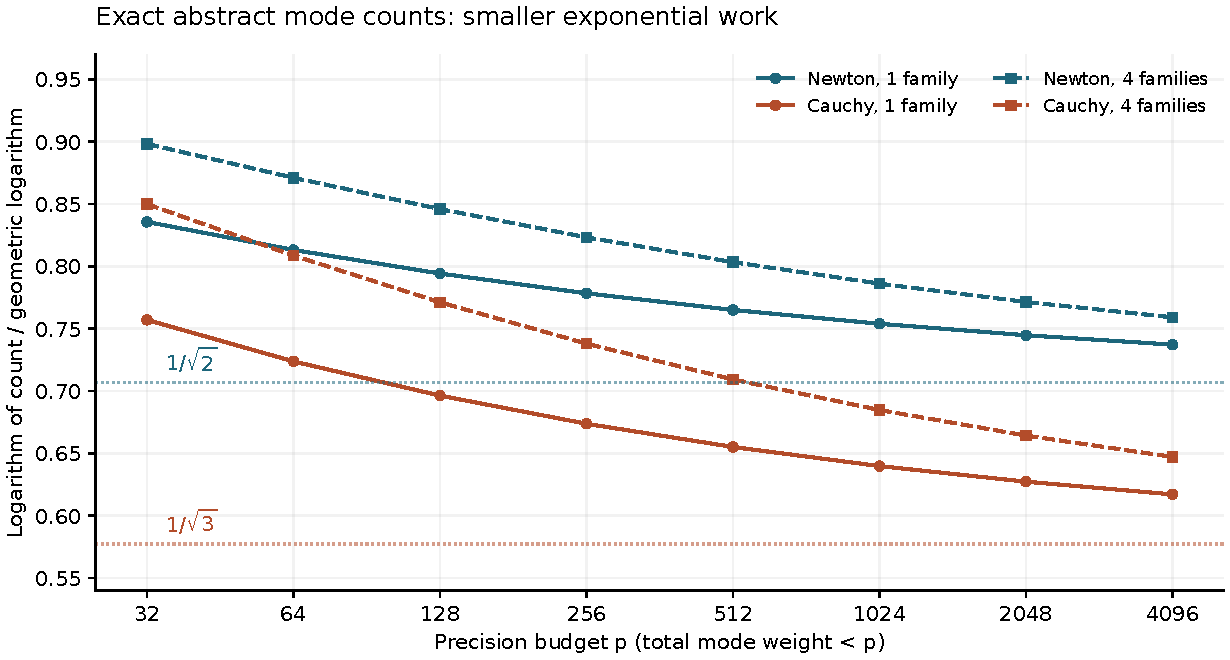
\includegraphics[width=.91\textwidth]{figures/mode_entropy.pdf}
\caption{Ratios of logarithms of exact abstract tuple counts. The horizontal limits are $1/\sqrt2$ and $1/\sqrt3$. These data concern enumeration counts, not complete SAT runtimes.}
\end{figure}

The proofs carry the asymptotic claims; finite checks do not prove them. Conversely, a mathematically correct replacement still needs integration into a full solver and, if desired, a new formalization effort before it inherits the original project's implementation or proof-assistant validation status.

\section{Why larger claimed improvements would be premature}\label{sec:limits}

\subsection{Linear valuation growth keeps the square-root exponent}

The new weights are asymptotically $3b$, still linear in the index. The generating function in Section~\ref{sec:entropy} therefore still has logarithm proportional to $1/\theta$. Optimizing $\theta p+A c/\theta$ still produces a square root. A different coefficient of $b$ improves the leading constant; it does not turn $M/\sqrt u$ into $M/u$.

Even elementary counting shows that the order cannot be removed merely by refining this particular enumeration bound. For $c\asymp M/D$, $p\asymp MD/u$, choose $B$ to be a sufficiently small constant times $D/\sqrt u$. The $cB$ variables with indices in $[B,2B)$ have weights $O(B)$. Every $0/1$ selection among them fits the budget after adjusting the constant, yielding $2^{\Omega(M/\sqrt u)}$ feasible tuples. Their total degree is at most $M$ for sufficiently large $u$. Thus adding the already available global monomial-degree cap does not eliminate this family.

\subsection{A Cauchy determinant checks the direction of improvement}

For the integral kernel $K(z,j)=1/(1-zj)$, take auxiliary rows $z=2a$ and columns $j=b$, with $0\le a,b<q$. Cauchy's determinant identity gives
\begin{equation}\label{eq:det-valuation}
 v_2(\det K)=\frac{q(q-1)}2+
            2\sum_{b=0}^{q-1}v_2(b!)=\Theta(q^2),
\end{equation}
because all denominators are odd. The successive pivots have valuation $b+2v_2(b!)\sim3b$, matching the present construction before the outer factor $c_x$.

This explains why factorial gains are available and why a proposal for generic quadratic valuation growth needs more than a new integral separated basis for the same kernel. For example, if a $q\times q$ matrix is an integral rank-$r$ product plus $2^hE$, multilinearity of the determinant makes its determinant divisible by $2^{h(q-r)}$. Apply this with $q=2r$ and \eqref{eq:det-valuation}: precision $h$ is only $O(r)$ on these test matrices. The auxiliary rows range over a larger domain than the actual reciprocal row parameters of a packet. Thus this is a restriction on uniform compression of that enlarged kernel family, not a lower bound for SAT or a prohibition on exploiting the narrower actual rows.

\subsection{The dense-formula logarithm has a separate cause}

The general-density reduction encodes selected test-variable incidences. Its retained incidence degree is $O(n)$, while the incidence universe can be $n\,\polylog n$. The resulting subset-index budget is $O(n\log\log n)$ \cite{reduction}. Replacing the local Cauchy basis does not change that representation.

Indexing only the union of the selected variables would use less information, but it would omit the allocation of contributions among tests. That missing allocation cannot simply be discarded: the coefficients depend on it. No efficient factorization that removes this cost has been established here. Likewise, selecting a constant sparsification density does not preserve the desired subexponential branching cost. Neither shortcut is used in the proposed theorem.

\subsection{What would count as a stronger next result}

A meaningful next target is an aggregation algorithm that evaluates the weighted mode sum without visiting all of its admissible tuples, with a rigorous bound that includes tensor degrees, entry evaluation, and inherited precision. Another is a counting-preserving reduction of general 3-CNF to $O(n)$ effective Boolean wires with affordable local entries. Either would attack an order-level obstruction left by this note. We do not assume such a result in any running-time claim.

\section{Integration plan and final assessment}

The implementation change is localized:
\begin{enumerate}[leftmargin=2em]
\item Keep the packet layout, interpolation nodes, taper, and group assignment.
\item At each crossing tile, compute $c_x,z_x$ and replace the powers $j^b$ by \eqref{eq:source-feature}.
\item Use \eqref{eq:target-feature} and certify its weight by Theorem~\ref{thm:weights}.
\item Enumerate only the tuples in \eqref{eq:weighted-budget}; preserve the original creation-precision semantics for packet tensors.
\item For the explicit global comparison, adopt the matched deeper cutoff \eqref{eq:newcutoff} and update the active-depth estimate.
\item Extend a full implementation's correctness checks to non-scalar interpolation values before making performance or formalization claims.
\end{enumerate}

The deliverable establishes a precise improvement of the existing algorithmic architecture: stronger integral mode coefficients, fewer exponentially many tuples, and a smaller explicit exponential upper-bound coefficient. The natural-language proof and prototype have been independently checked within this analysis, but external priority and novelty have not been established; the Cauchy identity itself is classical in character. Its useful contribution here is the exact fit to the source's interpolation domain and recursion.

If ``better asymptotic complexity'' is intended to require a new order such as $2^{o(n\log\log n/\sqrt{\log n})}$, this request is not resolved by the present result. The attached proofs distinguish that open objective from the improvement that is actually supported.

\begin{thebibliography}{9}
\raggedright
\bibitem{paper}
OpenAI, \emph{The Exponential Time Hypothesis is False}, October 17, 2026; revised October 25, 2026. Source at commit \texttt{7ef5c0cc5ca4b0e072b7a050fca09ab24bc6fa3a}.\par
\href{https://github.com/openai/math/tree/7ef5c0cc5ca4b0e072b7a050fca09ab24bc6fa3a/preprints/The-Exponential-Time-Hypothesis-is-False-October-25-2026}{Pinned manuscript directory}.

\bibitem{contraction}
OpenAI, \emph{Proof of the contraction theorem}, source file \texttt{quantitative-contraction.tex} in the same directory's \texttt{build/} folder. Relevant labels: \texttt{eq:tensor-mode-expansion}, \texttt{eq:tensor-mode-budget}, \texttt{eq:tensor-precision-bound}, and \texttt{eq:tensor-recursion-identity}.\par
\href{https://github.com/openai/math/blob/7ef5c0cc5ca4b0e072b7a050fca09ab24bc6fa3a/preprints/The-Exponential-Time-Hypothesis-is-False-October-25-2026/build/quantitative-contraction.tex}{Pinned contraction source}.

\bibitem{reduction}
OpenAI, \emph{A sharper bound for exact counting}, source file \texttt{quantitative-reduction.tex}, especially the incidence-degree and wire-budget encodings.\par
\href{https://github.com/openai/math/blob/7ef5c0cc5ca4b0e072b7a050fca09ab24bc6fa3a/preprints/The-Exponential-Time-Hypothesis-is-False-October-25-2026/build/quantitative-reduction.tex}{Pinned reduction source}.

\bibitem{scope}
OpenAI, \emph{The Exponential Time Hypothesis is False: scope of the Lean formalization}, \texttt{lean/docs/378.md}, accessed October 26, 2026.\par
\href{https://github.com/openai/math/blob/7ef5c0cc5ca4b0e072b7a050fca09ab24bc6fa3a/lean/docs/378.md}{Pinned scope document}.
\end{thebibliography}
\end{document}
